% !TeX program = lualatex
% Build from this directory with:
%   latexmk -lualatex -interaction=nonstopmode -halt-on-error -outdir=build poster.tex

\documentclass[final]{beamer}

\usepackage[size=a1,orientation=portrait,scale=1.0]{beamerposter}
\usepackage[british]{babel}
\usepackage{mathtools}
\usepackage{fontspec}
\defaultfontfeatures{Ligatures=TeX}
\setmainfont{STIX Two Text}
\setsansfont{STIX Two Text}
\newfontface\postersemibold{STIXTwoText-SemiBold.otf}
\usefonttheme{professionalfonts}
\usepackage[warnings-off={mathtools-colon,mathtools-overbracket}]{unicode-math}
\setmathfont{STIX Two Math}

\usepackage{microtype}
\usepackage{graphicx}
\usepackage{qrcode}
\usepackage{ragged2e}
\usepackage{tikz}
\usetikzlibrary{arrows.meta,positioning}

% -----------------------------------------------------------------------------
% Poster metadata: edit these lines first.
% -----------------------------------------------------------------------------
\title{Finding the \texorpdfstring{\(W\)}{W} in the Noise}
\subtitle{How collision data reveal a hidden particle signal}
\newcommand{\technicalsubtitle}{A data-driven analysis of \(W \to e\nu\) events with ATLAS Open Data}
\author{Giancarmine Sparso}
\institute{Department of Physics\\Sapienza University of Rome}
\newcommand{\contactline}{github.com/giancarmine-sparso}

% -----------------------------------------------------------------------------
% Structural poster palette.  Scientific plots retain their own magma palette;
% these colours are reserved for the poster interface and explanatory material.
% -----------------------------------------------------------------------------
\definecolor{OxfordBlue}{HTML}{0B1F3A}
\definecolor{YaleBlue}{HTML}{1E5A8A}
\definecolor{LightBlueGrey}{HTML}{E8EFF5}
\definecolor{WarmWhite}{HTML}{F8F9FA}
\definecolor{Graphite}{HTML}{202830}

\setbeamercolor{background canvas}{bg=WarmWhite}
\setbeamercolor{normal text}{fg=Graphite,bg=WarmWhite}
\setbeamercolor{structure}{fg=YaleBlue}
\setbeamercolor{alerted text}{fg=YaleBlue}
\setbeamercolor{headline}{fg=white,bg=OxfordBlue}
\setbeamercolor{headline accent}{fg=YaleBlue,bg=YaleBlue}
\setbeamercolor{footline}{fg=white,bg=OxfordBlue}
\setbeamercolor{poster title}{fg=white}
\setbeamercolor{poster subtitle}{fg=LightBlueGrey}
\setbeamercolor{poster technical subtitle}{fg=LightBlueGrey}
\setbeamercolor{poster author}{fg=white}
\setbeamercolor{poster institute}{fg=LightBlueGrey}
\setbeamercolor{block title}{fg=white,bg=OxfordBlue}
\setbeamercolor{block body}{fg=Graphite,bg=white}
\setbeamercolor{block title alerted}{fg=white,bg=OxfordBlue}
\setbeamercolor{block body alerted}{fg=Graphite,bg=LightBlueGrey}
\setbeamercolor{block title example}{fg=white,bg=OxfordBlue}
\setbeamercolor{block body example}{fg=Graphite,bg=LightBlueGrey}

% Explicit sizes keep the poster readable despite beamerposter's A-series scale.
\setbeamerfont{normal text}{size*={24pt}{30pt}}
\setbeamerfont{title}{size*={64pt}{72pt},series=\bfseries}
\setbeamerfont{subtitle}{size*={24pt}{30pt},series=\mdseries}
\setbeamerfont{technical subtitle}{size*={21pt}{26pt},series=\mdseries}
\setbeamerfont{author}{size*={32pt}{38pt},series=\mdseries,family=\postersemibold}
\setbeamerfont{institute}{size*={24pt}{30pt},series=\mdseries}
\setbeamerfont{block title}{size*={30pt}{36pt},series=\bfseries}
\setbeamerfont{block body}{size*={24pt}{30pt}}
\setbeamerfont{block title alerted}{parent=block title}
\setbeamerfont{block body alerted}{parent=block body}
\setbeamerfont{block title example}{parent=block title}
\setbeamerfont{block body example}{parent=block body}
\setbeamerfont{footline}{size*={24pt}{30pt},series=\mdseries}
\setbeamerfont{itemize/enumerate body}{size*={24pt}{30pt}}

\setbeamertemplate{navigation symbols}{}
\setbeamertemplate{blocks}[rounded][shadow=false]
\setbeamertemplate{itemize item}{\color{YaleBlue}\raisebox{0.12ex}{\small$\blacktriangleright$}}
\setbeamertemplate{itemize subitem}{\color{YaleBlue}\raisebox{0.12ex}{\scriptsize$\blacktriangleright$}}

% A restrained outer rule anchors the page without creating another blue area.
\setbeamertemplate{background}{%
  \begin{tikzpicture}[remember picture,overlay]
    \draw[OxfordBlue,line width=2pt]
      ([xshift=1pt,yshift=-1pt]current page.north west)
      rectangle
      ([xshift=-1pt,yshift=1pt]current page.south east);
  \end{tikzpicture}%
}

\newlength{\posterheadlineheight}
\newlength{\posterheadlinetopinset}
\newlength{\posterheadlineleftwidth}
\newlength{\posterheadlinerightwidth}
\newlength{\posterheadlineparagraphskip}
\newlength{\posterheadlineauthoroffset}
\setlength{\posterheadlineheight}{6.80cm}
\setlength{\posterheadlinetopinset}{1.55cm}
\setlength{\posterheadlineleftwidth}{0.63\paperwidth}
\setlength{\posterheadlinerightwidth}{0.29\paperwidth}
\setlength{\posterheadlineparagraphskip}{0.08cm}
% Compensates the different ascender heights so the first baselines coincide.
\setlength{\posterheadlineauthoroffset}{0.81cm}

\setbeamertemplate{headline}{%
  \begin{beamercolorbox}[wd=\paperwidth,sep=0pt]{headline}
    \begin{minipage}[t][\posterheadlineheight][t]{\paperwidth}
      \vspace*{\posterheadlinetopinset}%
      \noindent\hspace*{0.03\paperwidth}%
      \begin{minipage}[t]{\posterheadlineleftwidth}
        \raggedright
        \setlength{\parindent}{0pt}%
        \setlength{\parskip}{\posterheadlineparagraphskip}%
        {\usebeamerfont{title}\usebeamercolor[fg]{poster title}\inserttitle\par}
        {\usebeamerfont{subtitle}\usebeamercolor[fg]{poster subtitle}\insertsubtitle\par}
        {\usebeamerfont{technical subtitle}\usebeamercolor[fg]{poster technical subtitle}\technicalsubtitle\par}
      \end{minipage}%
      \hfill
      \raisebox{-\posterheadlineauthoroffset}[0pt][0pt]{%
        \begin{minipage}[t]{\posterheadlinerightwidth}
          \raggedleft
          \setlength{\parindent}{0pt}%
          \setlength{\parskip}{\posterheadlineparagraphskip}%
          {\usebeamerfont{author}\usebeamercolor[fg]{poster author}\insertauthor\par}
          {\usebeamerfont{institute}\usebeamercolor[fg]{poster institute}\insertinstitute\par}
        \end{minipage}%
      }%
      \hspace*{0.03\paperwidth}\par
    \end{minipage}%
  \end{beamercolorbox}%
  \begin{beamercolorbox}[wd=\paperwidth,ht=0.25cm,dp=0cm]{headline accent}\end{beamercolorbox}%
}

% The institutional marks sit in a compact three-part footer.
% Explicit heights keep the layout stable when the contact text changes.
\newlength{\posterfooterheight}
\newlength{\posterfooterlogoheight}
\newlength{\posterfooteratlasheight}
\newlength{\posterfooterlogogroupwidth}
\newlength{\posterfooterlogoseparation}
\newlength{\posterfootercontactgap}
\setlength{\posterfooterheight}{3.50cm}
\setlength{\posterfooterlogoheight}{2.50cm}
\setlength{\posterfooteratlasheight}{1.92cm}
\setlength{\posterfooterlogogroupwidth}{7.55cm}
\setlength{\posterfooterlogoseparation}{0.58cm}
\setlength{\posterfootercontactgap}{0.95cm}

\setbeamertemplate{footline}{%
  \leavevmode%
  \begin{beamercolorbox}[wd=\paperwidth,ht=\posterfooterheight,dp=0cm]{footline}%
    \vbox to \posterfooterheight{%
      \vfil
      \hbox to \paperwidth{%
        \hspace*{0.03\paperwidth}%
        \begin{minipage}[c]{\posterfooterlogogroupwidth}
          \raggedright
          \includegraphics[height=\posterfooterlogoheight]{%
            ../atlas-analysis/figures/oxford_crest_white_official_web.pdf}%
          \hspace{\posterfooterlogoseparation}%
          \includegraphics[height=\posterfooteratlasheight]{%
            ../atlas-analysis/figures/ATLAS-Logo-White-transparent.png}%
        \end{minipage}%
        \hspace{\posterfootercontactgap}%
        \begin{minipage}[c]{0.55\paperwidth}
          \raggedright
          \usebeamerfont{footline}\contactline
        \end{minipage}%
        \hfill
        \begin{minipage}[c]{0.12\paperwidth}
          \raggedleft
          
\includegraphics[
            height=\posterfooterlogoheight,
            trim=5bp 39bp 5bp 0bp,
            clip
          ]{../atlas-analysis/figures/lmh_crest_without_motto.pdf}%
        \end{minipage}%
        \hspace*{0.03\paperwidth}%
      }%
      \vfil
    }%
  \end{beamercolorbox}%
}

% Shared content grid.  Beamer's column boxes have a small visual overhang to
% the left, so the overlay row starts half a standard outer margin earlier.
% Its width and column widths remain identical to the main poster grid.
\newlength{\postercontentmargin}
\newlength{\postercontentwidth}
\newlength{\postermaincolumnwidth}
\setlength{\postercontentmargin}{0.015\paperwidth}
\setlength{\postercontentwidth}{0.94\paperwidth}
\setlength{\postermaincolumnwidth}{0.455\paperwidth}

\setlength{\parindent}{0pt}
\setlength{\parskip}{0.35cm}

% -----------------------------------------------------------------------------
% Reusable visual helpers.
% -----------------------------------------------------------------------------
\tikzset{
  poster flow node/.style={
    draw=YaleBlue,
    fill=LightBlueGrey,
    text=Graphite,
    line width=2pt,
    rounded corners=5pt,
    minimum height=3.2cm,
    text width=6.2cm,
    align=center,
    font=\bfseries
  },
  poster flow arrow/.style={
    -{Stealth[length=8mm,width=5mm]},
    draw=YaleBlue,
    line width=2.5pt
  }
}

\newcommand{\placeholdergraphic}[2][11cm]{%
  \begin{center}
    \begin{tikzpicture}
      \node[
        draw=YaleBlue,
        fill=LightBlueGrey,
        line width=1.5pt,
        rounded corners=5pt,
        minimum width=0.91\linewidth,
        minimum height=#1,
        text width=0.76\linewidth,
        align=center,
        text=Graphite
      ] {%
        {\fontsize{28pt}{34pt}\selectfont\bfseries #2}\par
        \vspace{0.5cm}
        {\fontsize{18pt}{23pt}\selectfont Replace this box with \textbackslash includegraphics.}%
      };
    \end{tikzpicture}
  \end{center}%
}

% Introductory event-display tile.  These lengths keep its geometry explicit
% while leaving the rest of the poster grid unchanged.
\newlength{\eventcontexttilewidth}
\newlength{\eventcontextpadding}
\newlength{\eventcontextimageheight}
\newlength{\eventcontextimagewidth}
\newlength{\eventcontextcaptionwidth}
\setlength{\eventcontexttilewidth}{0.42\paperwidth}
\setlength{\eventcontextpadding}{0.18cm}
\setlength{\eventcontextimageheight}{11.30cm}
\setlength{\eventcontextimagewidth}{0.288\paperwidth}
\setlength{\eventcontextcaptionwidth}{0.114\paperwidth}

% High-pile-up event display and its explanatory text panel.  Together they
% fill the reserved right-hand side of the introductory row without making it
% taller than the existing event-display tile.
\newlength{\pileupimagewidth}
\newlength{\pileuptextwidth}
\setlength{\pileupimagewidth}{\eventcontextimageheight}
\setlength{\pileuptextwidth}{0.2825\paperwidth}

\begin{document}

\begin{frame}[t]
  \usebeamerfont{normal text}
  \RaggedRight
  \vspace{0.9cm}

  % First content row: detector activity, pile-up, and its analysis consequence.
  \begin{columns}[t,totalwidth=\postercontentwidth]
    \begin{column}{\eventcontexttilewidth}
      \begin{block}{What does ATLAS see?}
        \hspace*{\eventcontextpadding}%
        \begin{minipage}[t][\eventcontextimageheight][t]{\eventcontextimagewidth}
          \vspace{0pt}%
          \centering
          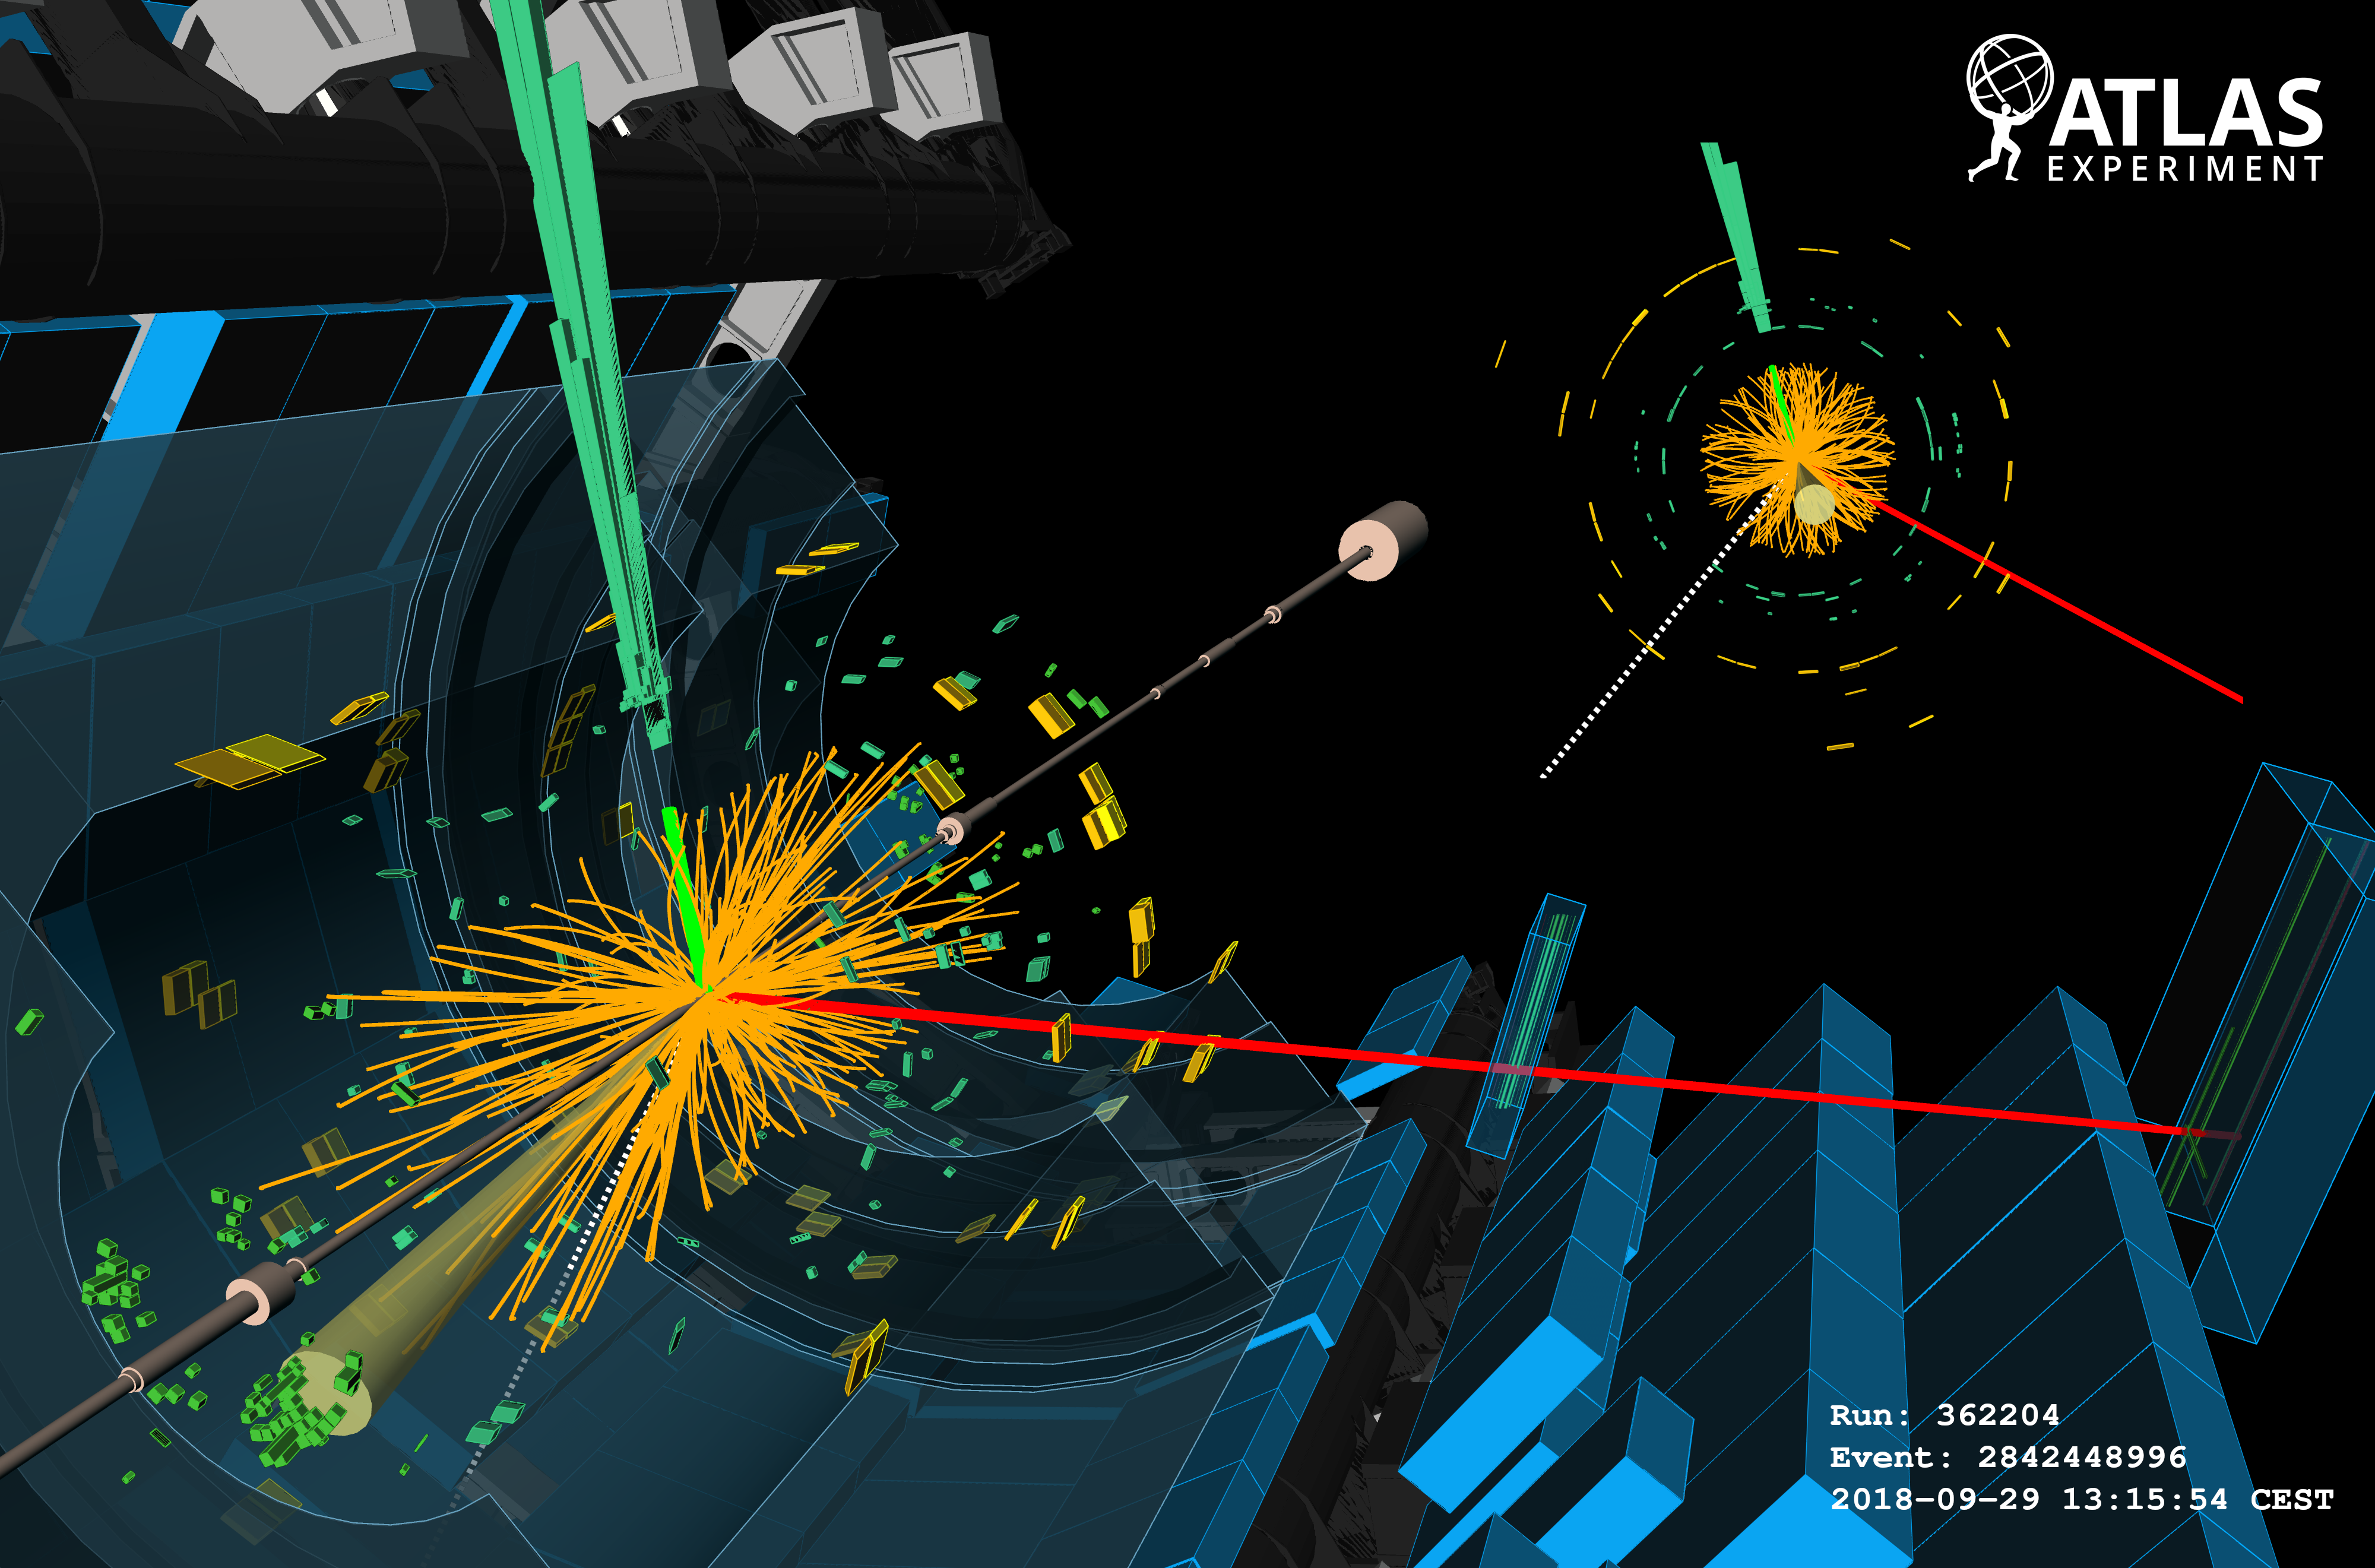
\includegraphics[
            width=\linewidth,
            height=\eventcontextimageheight,
            keepaspectratio,
            trim=0bp 0bp 0bp 0bp,
            clip
          ]{../atlas-analysis/figures/atlas_event_display.png}%
        \end{minipage}%
        \hfill
        \begin{minipage}[t][\eventcontextimageheight][c]{\eventcontextcaptionwidth}
          \vspace{0pt}%
          \raggedright
          \usebeamerfont{normal text}%
          \fontsize{22pt}{28pt}\selectfont
          \color{Graphite}%
          \setlength{\parskip}{0pt}%
          \hyphenpenalty=10000%
          \exhyphenpenalty=10000%
          Each collision produces \textbf{many particles at once}. We search
          for one \textbf{electron} and an \textbf{invisible neutrino} within
          this activity.\textsuperscript{[1]}%
        \end{minipage}%
        \hspace*{\eventcontextpadding}%
      \end{block}
    \end{column}

    \begin{column}{0.49\paperwidth}
      \begin{block}{Why is the signal hard to isolate?}
        \hspace*{\eventcontextpadding}%
        \begin{minipage}[t][\eventcontextimageheight][t]{\pileupimagewidth}
          \vspace{0pt}%
          \centering
          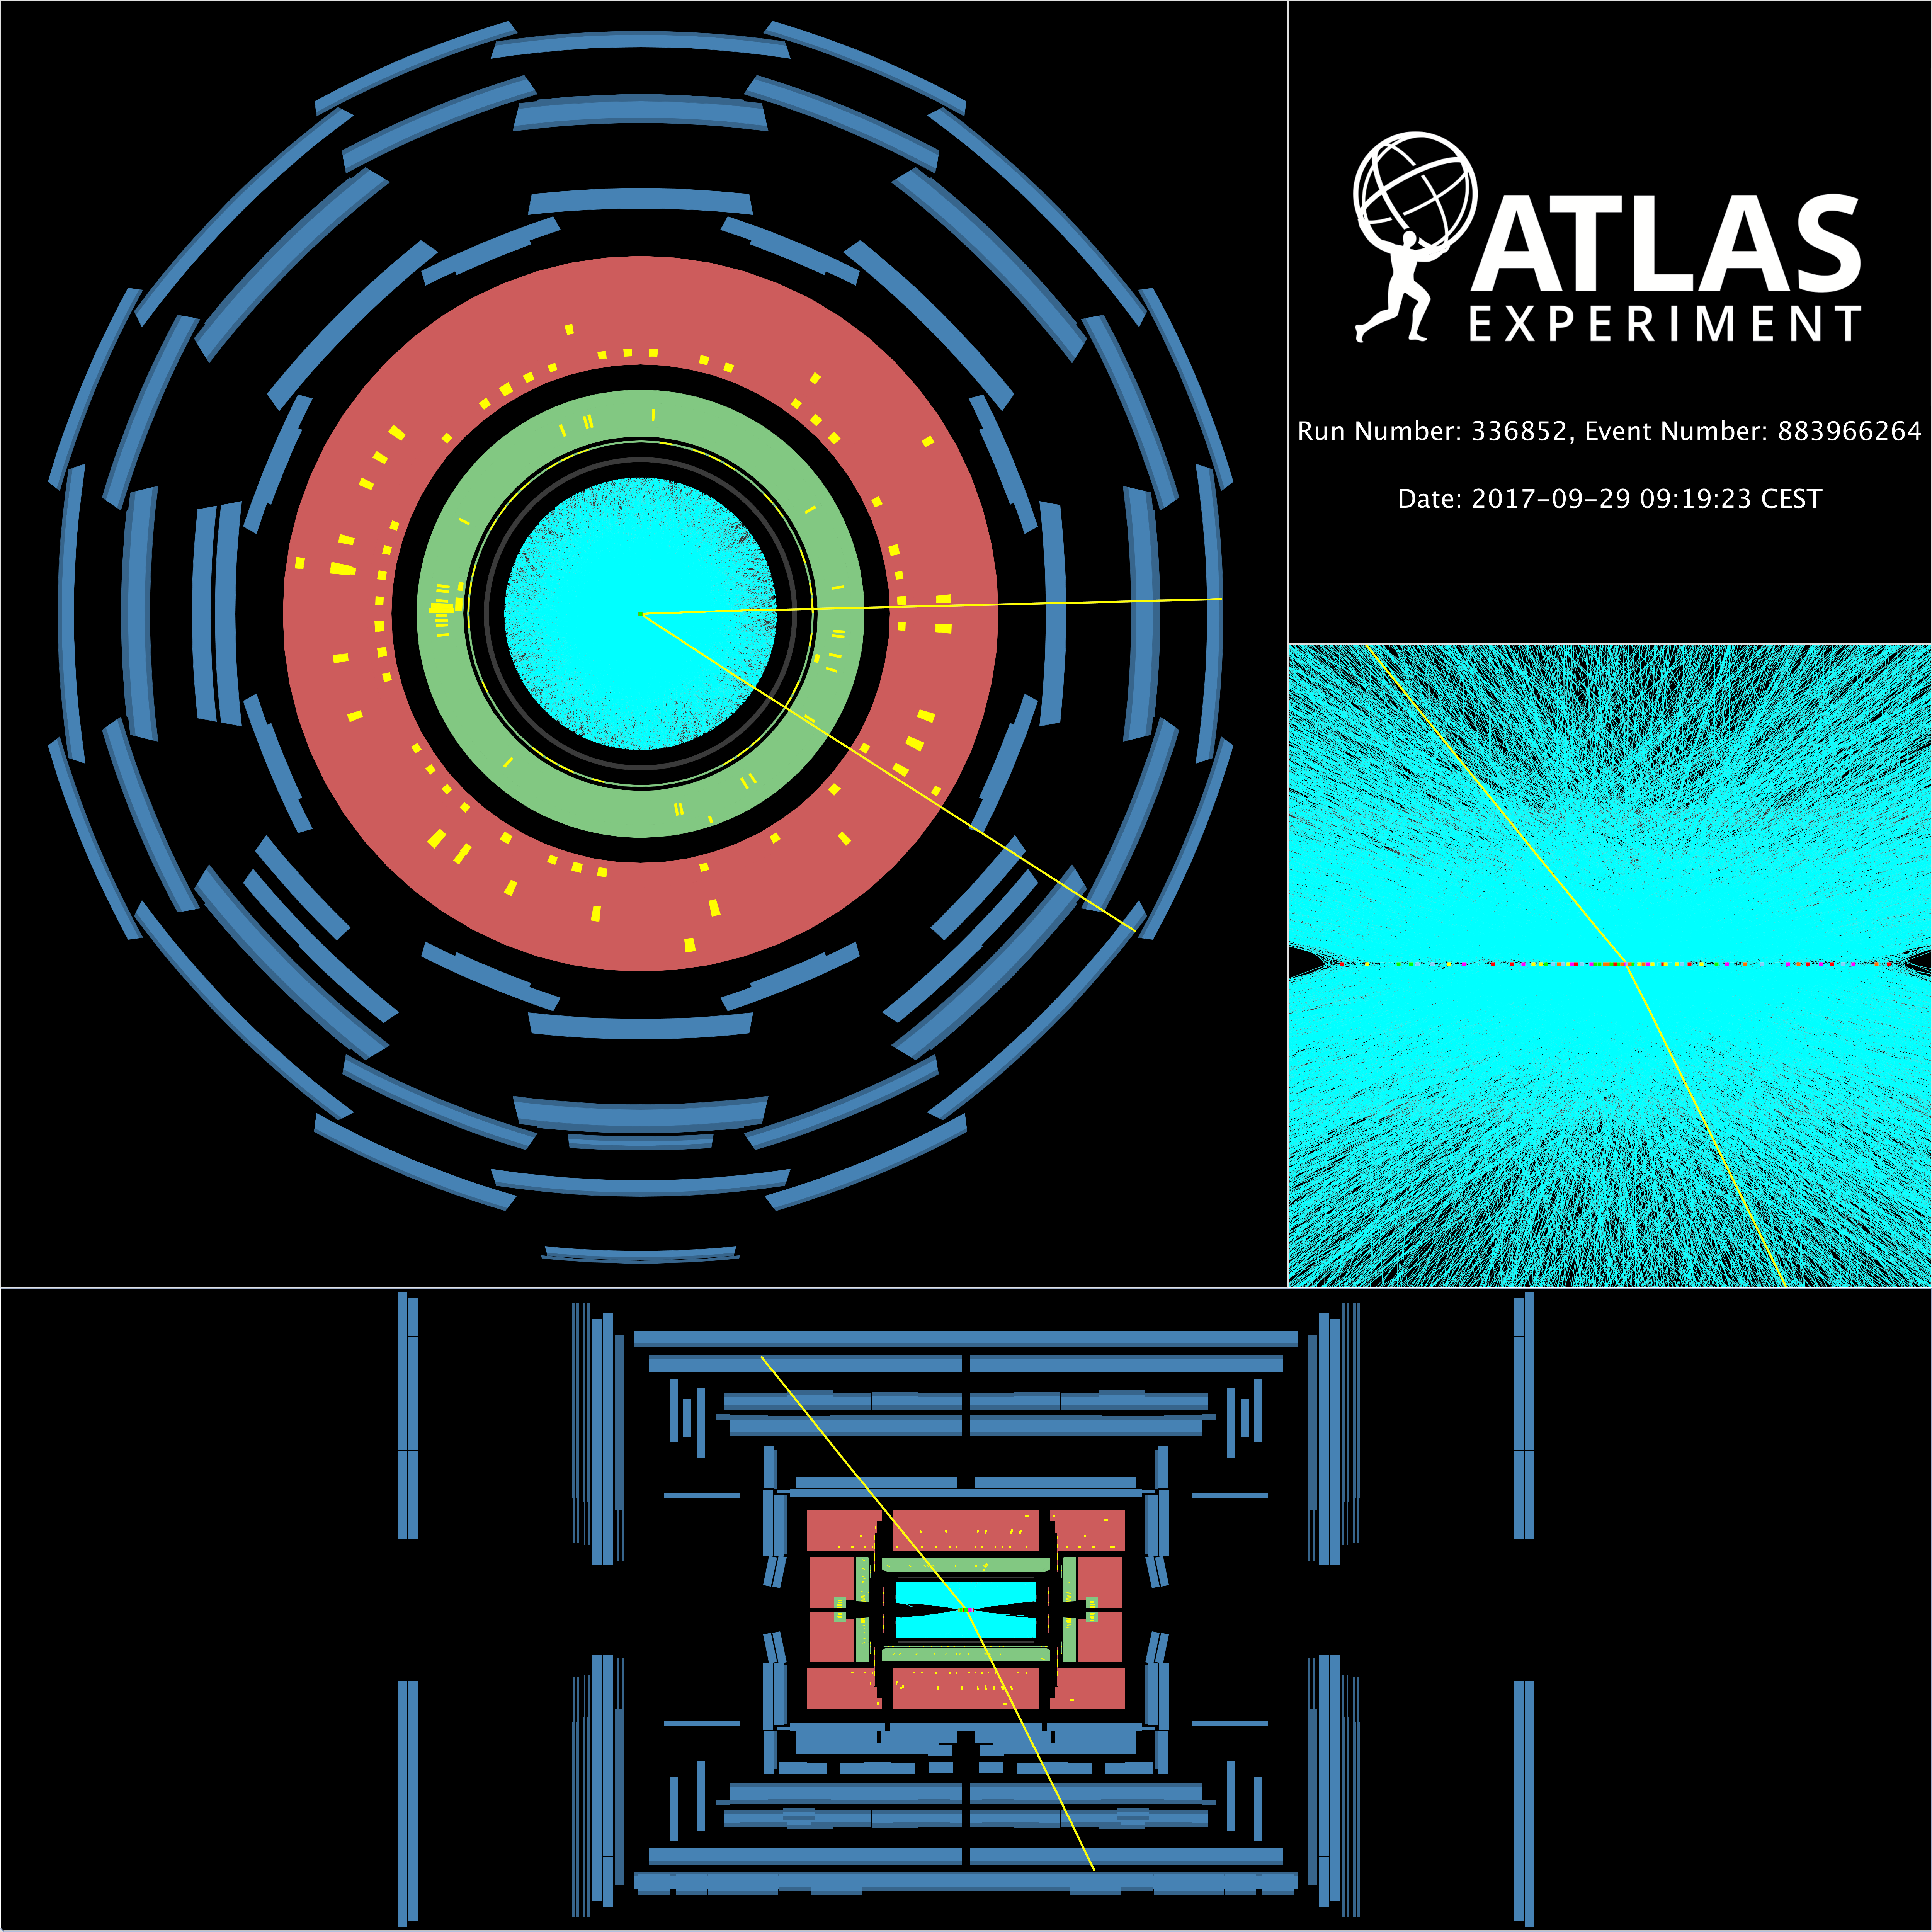
\includegraphics[
            width=\linewidth,
            height=\eventcontextimageheight,
            keepaspectratio,
            trim=3333bp 1666bp 0bp 1667bp,
            clip
          ]{../atlas-analysis/figures/zpileup_alltracks.png}%
        \end{minipage}%
        \hfill
        \begin{minipage}[t][\eventcontextimageheight][c]{\pileuptextwidth}
          \vspace{0pt}%
          \raggedright
          \usebeamerfont{normal text}%
          \fontsize{24pt}{30pt}\selectfont
          \color{Graphite}%
          \setlength{\parskip}{0pt}%
          \hyphenpenalty=10000%
          \exhyphenpenalty=10000%
          One recorded event can contain dozens of overlapping proton--proton
          collisions.\par
          Here, ATLAS reconstructed \textbf{66 collision vertices}: 1 produced
          the highlighted \(Z \to \mu^+\mu^-\) candidate, while the other
          \textbf{65 are pile-up}.\par
          Their overlapping tracks and energy obscure the \(W \to e\nu\)
          signature.\textsuperscript{[2]}%
        \end{minipage}%
        \hspace*{\eventcontextpadding}%
      \end{block}
    \end{column}
  \end{columns}

  \vspace{0.30cm}

  \begin{columns}[t,totalwidth=\postercontentwidth]
    \begin{column}{\postermaincolumnwidth}

      \begin{block}{Event Selection}
        \vspace*{0.20cm}
        {\fontsize{26pt}{32pt}\selectfont
          Four requirements progressively isolate the signature of
          \(W \rightarrow e\nu\): one visible electron and momentum carried away
          by an invisible neutrino.\par
        }

        \vspace{0.45cm}

        \centering
        \begin{tikzpicture}[
          selection marker/.style={
            circle,
            draw=YaleBlue,
            fill=white,
            text=YaleBlue,
            line width=2pt,
            minimum size=1.45cm,
            inner sep=0pt,
            font=\fontsize{28pt}{32pt}\selectfont\bfseries
          },
          selection detail/.style={
            anchor=north west,
            text=Graphite,
            text width=0.83\linewidth,
            inner sep=0pt,
            align=left
          },
          selection spine/.style={
            draw=YaleBlue,
            line width=2pt
          },
          selection final/.style={
            anchor=north west,
            draw=YaleBlue,
            fill=LightBlueGrey,
            text=Graphite,
            line width=1.5pt,
            rounded corners=5pt,
            minimum width=0.91\linewidth,
            minimum height=3.35cm,
            text width=0.84\linewidth,
            inner xsep=0.55cm,
            inner ysep=0.28cm,
            align=left
          }
        ]
          \coordinate (point-one) at (0,0);
          \coordinate (point-two) at (0,-4.90cm);
          \coordinate (point-three) at (0,-9.80cm);
          \coordinate (point-four) at (0,-14.70cm);

          \draw[selection spine] (point-one) -- (point-four);

          \node[selection marker] (marker-one) at (point-one) {1};
          \node[selection marker] (marker-two) at (point-two) {2};
          \node[selection marker] (marker-three) at (point-three) {3};
          \node[selection marker] (marker-four) at (point-four) {4};

          \node[selection detail] (step-one)
            at ([xshift=0.65cm,yshift=0.56cm]marker-one.east) {%
              \begin{minipage}[t]{0.64\linewidth}
                \raggedright
                {\fontsize{25pt}{30pt}\selectfont\bfseries One electron candidate}
              \end{minipage}%
              \hfill
              \begin{minipage}[t]{0.33\linewidth}
                \raggedleft
                {\color{OxfordBlue}\fontsize{22pt}{27pt}\selectfont
                  \(p_T^e > 25\,\mathrm{GeV}\)}
              \end{minipage}\par
              \vspace{0.14cm}
              {\fontsize{22pt}{27pt}\selectfont
                Identifies the visible particle produced in the \(W\) decay.\par}
              \vspace{0.20cm}
              \begin{minipage}[c]{0.64\linewidth}
                \raggedright
                \begin{tikzpicture}[baseline=-0.12cm]
                  \fill[LightBlueGrey,rounded corners=2pt]
                    (0,0) rectangle (12.0cm,0.42cm);
                  \fill[YaleBlue,rounded corners=2pt]
                    (0,0) rectangle (12.0cm,0.42cm);
                \end{tikzpicture}%
              \end{minipage}%
              \hfill
              \begin{minipage}[c]{0.33\linewidth}
                \raggedleft
                {\fontsize{22pt}{26pt}\selectfont\bfseries
                  5.39M events (100\%)}
              \end{minipage}%
            };

          \node[selection detail] (step-two)
            at ([xshift=0.65cm,yshift=0.56cm]marker-two.east) {%
              \begin{minipage}[t]{0.72\linewidth}
                \raggedright
                {\fontsize{25pt}{30pt}\selectfont\bfseries
                  Tight electron identification}
              \end{minipage}%
              \hfill
              \begin{minipage}[t]{0.25\linewidth}
                \raggedleft
                {\color{OxfordBlue}\fontsize{22pt}{27pt}\selectfont Tight ID}
              \end{minipage}\par
              \vspace{0.14cm}
              {\fontsize{22pt}{27pt}\selectfont
                Rejects jets mistakenly reconstructed as electrons.\par}
              \vspace{0.20cm}
              \begin{minipage}[c]{0.64\linewidth}
                \raggedright
                \begin{tikzpicture}[baseline=-0.12cm]
                  \fill[LightBlueGrey,rounded corners=2pt]
                    (0,0) rectangle (12.0cm,0.42cm);
                  \fill[YaleBlue,rounded corners=2pt]
                    (0,0) rectangle (10.49cm,0.42cm);
                \end{tikzpicture}%
              \end{minipage}%
              \hfill
              \begin{minipage}[c]{0.33\linewidth}
                \raggedleft
                {\fontsize{22pt}{26pt}\selectfont\bfseries
                  4.71M events (87\%)}
              \end{minipage}%
            };

          \node[selection detail] (step-three)
            at ([xshift=0.65cm,yshift=0.56cm]marker-three.east) {%
              \begin{minipage}[t]{0.48\linewidth}
                \raggedright
                {\fontsize{25pt}{30pt}\selectfont\bfseries Electron isolation}
              \end{minipage}%
              \hfill
              \begin{minipage}[t]{0.49\linewidth}
                \raggedleft
                {\color{OxfordBlue}\fontsize{22pt}{27pt}\selectfont
                  \(p_T^{\mathrm{cone30}}/p_T^e < 0.10\)}
              \end{minipage}\par
              \vspace{0.14cm}
              {\fontsize{22pt}{27pt}\selectfont
                Removes electron-like candidates produced inside hadronic jets.\par}
              \vspace{0.20cm}
              \begin{minipage}[c]{0.64\linewidth}
                \raggedright
                \begin{tikzpicture}[baseline=-0.12cm]
                  \fill[LightBlueGrey,rounded corners=2pt]
                    (0,0) rectangle (12.0cm,0.42cm);
                  \fill[YaleBlue,rounded corners=2pt]
                    (0,0) rectangle (9.89cm,0.42cm);
                \end{tikzpicture}%
              \end{minipage}%
              \hfill
              \begin{minipage}[c]{0.33\linewidth}
                \raggedleft
                {\fontsize{22pt}{26pt}\selectfont\bfseries
                  4.45M events (82\%)}
              \end{minipage}%
            };

          \node[selection detail] (step-four)
            at ([xshift=0.65cm,yshift=0.56cm]marker-four.east) {%
              \begin{minipage}[t]{0.64\linewidth}
                \raggedright
                {\fontsize{25pt}{30pt}\selectfont\bfseries
                  Missing transverse momentum}
              \end{minipage}%
              \hfill
              \begin{minipage}[t]{0.33\linewidth}
                \raggedleft
                {\color{OxfordBlue}\fontsize{22pt}{27pt}\selectfont
                  \(E_T^{\mathrm{miss}} > 30\,\mathrm{GeV}\)}
              \end{minipage}\par
              \vspace{0.14cm}
              {\fontsize{22pt}{27pt}\selectfont
                Selects events compatible with an invisible neutrino.\par}
              \vspace{0.20cm}
              \begin{minipage}[c]{0.64\linewidth}
                \raggedright
                \begin{tikzpicture}[baseline=-0.12cm]
                  \fill[LightBlueGrey,rounded corners=2pt]
                    (0,0) rectangle (12.0cm,0.42cm);
                  \fill[YaleBlue,rounded corners=2pt]
                    (0,0) rectangle (5.54cm,0.42cm);
                \end{tikzpicture}%
              \end{minipage}%
              \hfill
              \begin{minipage}[c]{0.33\linewidth}
                \raggedleft
                {\fontsize{22pt}{26pt}\selectfont\bfseries
                  2.49M events (46\%)}
              \end{minipage}%
            };

          \node[selection final] (selected-sample)
            at ([xshift=-0.72cm,yshift=-3.45cm]marker-four.center) {%
              {\fontsize{25pt}{30pt}\selectfont\bfseries Selected sample\par}
              \vspace{0.10cm}
              {\fontsize{23pt}{28pt}\selectfont
                A background-reduced sample enriched in
                \(W \rightarrow e\nu\) candidates, ready for the transverse-mass
                analysis.}
            };

          \draw[-{Stealth[length=3.5mm,width=2.6mm]},draw=YaleBlue,line width=2pt]
            (marker-four.south) --
            ([xshift=0.72cm,yshift=0.25cm]selected-sample.north west);
        \end{tikzpicture}
      \end{block}

      \vspace{0.45cm}

      \begin{block}{Effect of the Selection}
        \centering
        \includegraphics[width=\linewidth]{%
          ../atlas-analysis/plots/final/mt_broad_sample.pdf}%

        \vspace{0.18cm}

        \includegraphics[width=\linewidth]{%
          ../atlas-analysis/plots/final/mt_selected_sample.pdf}%

        \vspace{0.10cm}

        \RaggedRight
        {\fontsize{21pt}{26pt}\selectfont
          The selection suppresses the low-\(m_T\) component and reveals the
          characteristic \(W\)-like structure near \(80\,\mathrm{GeV}\).\par
        }
      \end{block}

    \end{column}

    \begin{column}{\postermaincolumnwidth}

      \begin{block}{ABCD Method}
        \vspace*{0.25cm}

        \RaggedRight
        \hyphenpenalty=10000
        \exhyphenpenalty=10000
        {\fontsize{24pt}{30pt}\selectfont
          The aim is to estimate how many background events enter the signal
          region using the data themselves. Events are classified using two
          variables:\par

          \vspace{0.18cm}

          \textbf{Electron isolation} measures activity around the electron
          candidate. \textbf{Missing transverse momentum} measures the detector's
          momentum imbalance. A large \(E_T^{\mathrm{miss}}\) is compatible with
          an invisible neutrino.\par

          \vspace{0.18cm}

          Together, these variables define four regions:\par

          \vspace{0.12cm}

          \begin{minipage}[t]{0.48\linewidth}
            \vspace{0pt}
            \textbf{A --- signal region}\par
            Isolated electron, high \(E_T^{\mathrm{miss}}\).
          \end{minipage}%
          \hfill
          \begin{minipage}[t]{0.48\linewidth}
            \vspace{0pt}
            \textbf{B --- control region}\par
            Non-isolated electron, high \(E_T^{\mathrm{miss}}\).
          \end{minipage}\par

          \vspace{0.16cm}

          \begin{minipage}[t]{0.48\linewidth}
            \vspace{0pt}
            \textbf{C --- control region}\par
            Isolated electron, low \(E_T^{\mathrm{miss}}\).
          \end{minipage}%
          \hfill
          \begin{minipage}[t]{0.48\linewidth}
            \vspace{0pt}
            \textbf{D --- background-rich region}\par
            Non-isolated electron, low \(E_T^{\mathrm{miss}}\).
          \end{minipage}\par

          \vspace{0.22cm}

          For multijet background, electron isolation and
          \(E_T^{\mathrm{miss}}\) are assumed to be approximately independent.
          Thus, the isolated-to-non-isolated ratio should be similar at high and
          low \(E_T^{\mathrm{miss}}\):\par
        }

        {\fontsize{24pt}{30pt}\selectfont
          \[
            \frac{N_A^{\mathrm{bkg}}}{N_B^{\mathrm{bkg}}}
            \approx
            \frac{N_C^{\mathrm{bkg}}}{N_D^{\mathrm{bkg}}}
            \quad\Longrightarrow\quad
            N_{A,\mathrm{pred}}^{\mathrm{bkg}}
            \approx
            \frac{N_B^{\mathrm{bkg}}N_C^{\mathrm{bkg}}}
                 {N_D^{\mathrm{bkg}}}
          \]
        }

        {\fontsize{24pt}{30pt}\selectfont
          Regions B, C and D therefore act as control samples; their populations
          predict the background in the signal-like region A.\par
        }

        \vspace{0.12cm}

        \centering
        \includegraphics[width=\linewidth]{%
          ../atlas-analysis/plots/final/abcd_plane_data.pdf}%
      \end{block}

      \vspace{0.05cm}

      \begin{exampleblock}{Conclusions}
        \vspace*{0.03cm}
        \begin{minipage}[t][8.7cm][s]{\linewidth}
          \vspace{0pt}
          \RaggedRight
          {\setbeamerfont{itemize/enumerate body}{size*={27pt}{34pt}}%
            \begin{itemize}
              \setlength{\itemsep}{0.20cm}
              \setlength{\parskip}{0pt}
              \item Electron ID, isolation and \(E_T^{\mathrm{miss}}\) suppress
                the low-\(m_T\) background.
              \item ABCD predicts
                \((0.525 \pm 0.008_{\mathrm{stat}})\,\mathrm{M}\) background
                events in A; \(2.112\,\mathrm{M}\) are observed.
              \item Selection reveals the \(W \to e\nu\) transverse-mass
                structure near \(80\,\mathrm{GeV}\).
            \end{itemize}
          }
          \vfill
          {\fontsize{18pt}{22pt}\selectfont\itshape
            Preliminary data-only estimate: the ABCD excess is not yet a
            measured \(W\) yield.\par
          }
        \end{minipage}
        \vspace*{0.01cm}
      \end{exampleblock}
    \end{column}
  \end{columns}

  \begin{tikzpicture}[remember picture,overlay]
    \node[
      anchor=south west,
      inner sep=0pt,
      outer sep=0pt
    ] at ([
      xshift=\postercontentmargin,
      yshift=\dimexpr\posterfooterheight+0.45cm\relax
    ]current page.south west) {%
      \begin{minipage}[b][3.5cm][c]{\postercontentwidth}
        \begin{minipage}[c][3.5cm][c]{\postermaincolumnwidth}
          \RaggedRight
          \hyphenpenalty=10000
          \exhyphenpenalty=10000
          \setlength{\parskip}{0pt}
          {\fontsize{20pt}{23pt}\selectfont
            \textbf{References \& acknowledgements}\par
          }
          \vspace{0.10cm}
          {\fontsize{18pt}{21pt}\selectfont
            [1] ATLAS Coll., ``ATLAS event display'', CDS 2842773.\par
            [2] ATLAS Coll., \(Z \to \mu^+\mu^-\) candidate with 65 additional
            vertices (2017).\par
            Analysis based on ATLAS Open Data.\par
          }
        \end{minipage}%
        \hfill
        \begin{minipage}[c][3.5cm][c]{\postermaincolumnwidth}
          \raggedleft
          \begin{minipage}[c]{4.0cm}
            \centering
            {\fontsize{18pt}{21pt}\selectfont\bfseries Repository\par}
          \end{minipage}%
          \hspace{0.4cm}%
          \begin{minipage}[c]{3.5cm}
            \centering
            \qrcode[height=3.5cm]{https://github.com/giancarmine-sparso/lmh-oxford-phys02}%
          \end{minipage}%
        \end{minipage}%
      \end{minipage}%
    };
  \end{tikzpicture}

\end{frame}

\end{document}
